\chapter{پرسش‌های درختی}

\index{tree query@پرسش درختی}

این فصل روش‌های پردازش پرسش‌ها روی زیردرخت‌ها و مسیرهای یک درخت ریشه‌دار را بررسی می‌کند.
برای نمونه، چنین پرسش‌هایی عبارتند از:

\begin{itemize}
\item $k$امین نیاکان یک گره چیست؟
\item مجموع مقادیر در زیردرخت یک گره چقدر است؟
\item مجموع مقادیر روی مسیر بین دو گره چقدر است؟
\item کمترین جد مشترک دو گره کدام است؟
\end{itemize}

\section{یافتن نیاکان}

\index{ancestor@نیاکان}

$k$امین \key{نیاکان} گره $x$ در درخت ریشه‌دار، گره‌ای است که با پیمودن $k$ سطح به سمت بالا از $x$ به آن می‌رسیم.
فرض کنید $\texttt{ancestor}(x,k)$ نشان‌دهنده $k$امین نیاکان گره $x$ باشد (یا $0$ اگر چنین نیاکانی وجود نداشته باشد).
برای نمونه، در درخت زیر، $\texttt{ancestor}(2,1)=1$ و $\texttt{ancestor}(8,2)=4$ است.
\begin{center}
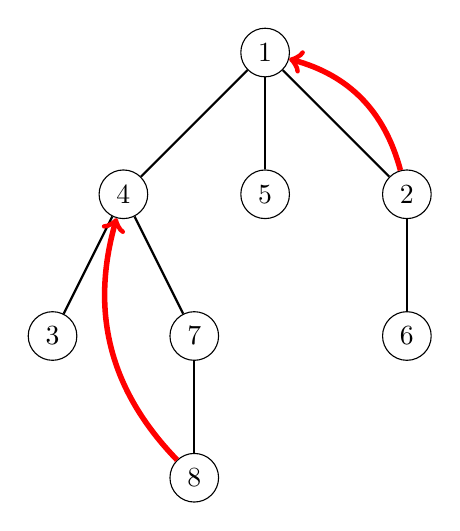
\begin{tikzpicture}[scale=0.9]
\node[draw, circle] (1) at (0,3) {$1$};
\node[draw, circle] (2) at (2,1) {$2$};
\node[draw, circle] (3) at (-2,1) {$4$};
\node[draw, circle] (4) at (0,1) {$5$};
\node[draw, circle] (5) at (2,-1) {$6$};
\node[draw, circle] (6) at (-3,-1) {$3$};
\node[draw, circle] (7) at (-1,-1) {$7$};
\node[draw, circle] (8) at (-1,-3) {$8$};
\path[draw,thick,-] (1) -- (2);
\path[draw,thick,-] (1) -- (3);
\path[draw,thick,-] (1) -- (4);
\path[draw,thick,-] (2) -- (5);
\path[draw,thick,-] (3) -- (6);
\path[draw,thick,-] (3) -- (7);
\path[draw,thick,-] (7) -- (8);

\path[draw=red,thick,->,line width=2pt] (8) edge [bend left] (3);
\path[draw=red,thick,->,line width=2pt] (2) edge [bend right] (1);
\end{tikzpicture}
\end{center}

روشی ساده برای محاسبه هر مقدار $\texttt{ancestor}(x,k)$، پیمودن $k$ گام متوالی در درخت است.
پیچیدگی زمانی این روش $O(k)$ است و امکان دارد کند باشد، زیرا درختی با $n$ گره ممکن است شامل زنجیری از $n$ گره باشد.

با تکنیکی مشابه روش فصل ۱۶.۳، پس از پیش‌پردازش، هر مقدار $\texttt{ancestor}(x,k)$ در زمان $O(\log k)$ قابل محاسبه است.
ایده کار، پیش‌محاسبه تمام مقادیر $\texttt{ancestor}(x,k)$ است که در آن $k \le n$ توانی از دو باشد.
برای نمونه، مقادیر درخت بالا چنین است:

\begin{center}
\begin{tabular}{r|rrrrrrrrr}
$x$ & 1 & 2 & 3 & 4 & 5 & 6 & 7 & 8 \\
\hline
$\texttt{ancestor}(x,1)$ & 0 & 1 & 4 & 1 & 1 & 2 & 4 & 7 \\
$\texttt{ancestor}(x,2)$ & 0 & 0 & 1 & 0 & 0 & 1 & 1 & 4 \\
$\texttt{ancestor}(x,4)$ & 0 & 0 & 0 & 0 & 0 & 0 & 0 & 0 \\
$\cdots$ \\
\end{tabular}
\end{center}

پیش‌پردازش نیازمند زمان $O(n \log n)$ است، زیرا برای هر گره $O(\log n)$ مقدار محاسبه می‌شود.
سپس، هر مقدار $\texttt{ancestor}(x,k)$ با نمایش $k$ به عنوان مجموع توان‌هایی از دو، در زمان $O(\log k)$ محاسبه می‌شود.

\section{زیردرخت‌ها و مسیرها}

\index{tree traversal array@آرایه پیمایش درخت}

یک \key{آرایه پیمایش درخت} گره‌های یک درخت ریشه‌دار را به ترتیبی نگه می‌دارد که جستجوی اول عمق از گره ریشه آن‌ها را ملاقات می‌کند.
برای مثال، در درخت
\begin{center}
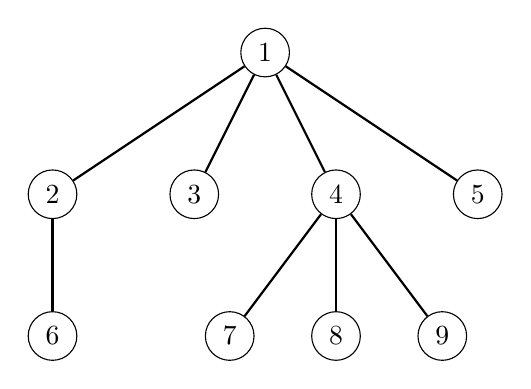
\begin{tikzpicture}[scale=0.9]
\node[draw, circle] (1) at (0,3) {$1$};
\node[draw, circle] (2) at (-3,1) {$2$};
\node[draw, circle] (3) at (-1,1) {$3$};
\node[draw, circle] (4) at (1,1) {$4$};
\node[draw, circle] (5) at (3,1) {$5$};
\node[draw, circle] (6) at (-3,-1) {$6$};
\node[draw, circle] (7) at (-0.5,-1) {$7$};
\node[draw, circle] (8) at (1,-1) {$8$};
\node[draw, circle] (9) at (2.5,-1) {$9$};

\path[draw,thick,-] (1) -- (2);
\path[draw,thick,-] (1) -- (3);
\path[draw,thick,-] (1) -- (4);
\path[draw,thick,-] (1) -- (5);
\path[draw,thick,-] (2) -- (6);
\path[draw,thick,-] (4) -- (7);
\path[draw,thick,-] (4) -- (8);
\path[draw,thick,-] (4) -- (9);
\end{tikzpicture}
\end{center}
یک جستجوی اول عمق به این صورت پیش می‌رود:
\begin{center}
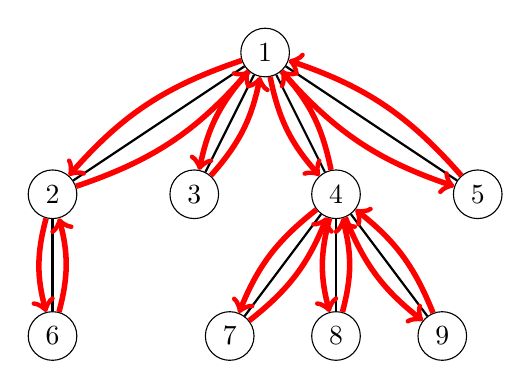
\begin{tikzpicture}[scale=0.9]
\node[draw, circle] (1) at (0,3) {$1$};
\node[draw, circle] (2) at (-3,1) {$2$};
\node[draw, circle] (3) at (-1,1) {$3$};
\node[draw, circle] (4) at (1,1) {$4$};
\node[draw, circle] (5) at (3,1) {$5$};
\node[draw, circle] (6) at (-3,-1) {$6$};
\node[draw, circle] (7) at (-0.5,-1) {$7$};
\node[draw, circle] (8) at (1,-1) {$8$};
\node[draw, circle] (9) at (2.5,-1) {$9$};

\path[draw,thick,-] (1) -- (2);
\path[draw,thick,-] (1) -- (3);
\path[draw,thick,-] (1) -- (4);
\path[draw,thick,-] (1) -- (5);
\path[draw,thick,-] (2) -- (6);
\path[draw,thick,-] (4) -- (7);
\path[draw,thick,-] (4) -- (8);
\path[draw,thick,-] (4) -- (9);


\path[draw=red,thick,->,line width=2pt] (1) edge [bend right=15] (2);
\path[draw=red,thick,->,line width=2pt] (2) edge [bend right=15] (6);
\path[draw=red,thick,->,line width=2pt] (6) edge [bend right=15] (2);
\path[draw=red,thick,->,line width=2pt] (2) edge [bend right=15] (1);
\path[draw=red,thick,->,line width=2pt] (1) edge [bend right=15] (3);
\path[draw=red,thick,->,line width=2pt] (3) edge [bend right=15] (1);
\path[draw=red,thick,->,line width=2pt] (1) edge [bend right=15] (4);
\path[draw=red,thick,->,line width=2pt] (4) edge [bend right=15] (7);
\path[draw=red,thick,->,line width=2pt] (7) edge [bend right=15] (4);
\path[draw=red,thick,->,line width=2pt] (4) edge [bend right=15] (8);
\path[draw=red,thick,->,line width=2pt] (8) edge [bend right=15] (4);
\path[draw=red,thick,->,line width=2pt] (4) edge [bend right=15] (9);
\path[draw=red,thick,->,line width=2pt] (9) edge [bend right=15] (4);
\path[draw=red,thick,->,line width=2pt] (4) edge [bend right=15] (1);
\path[draw=red,thick,->,line width=2pt] (1) edge [bend right=15] (5);
\path[draw=red,thick,->,line width=2pt] (5) edge [bend right=15] (1);

\end{tikzpicture}
\end{center}
بنابراین، آرایه پیمایش درخت متناظر به شرح زیر است:
\begin{center}
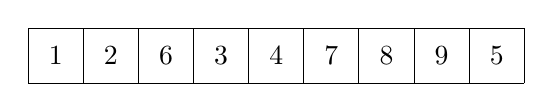
\begin{tikzpicture}[scale=0.7]
\draw (0,0) grid (9,1);

\node at (0.5,0.5) {$1$};
\node at (1.5,0.5) {$2$};
\node at (2.5,0.5) {$6$};
\node at (3.5,0.5) {$3$};
\node at (4.5,0.5) {$4$};
\node at (5.5,0.5) {$7$};
\node at (6.5,0.5) {$8$};
\node at (7.5,0.5) {$9$};
\node at (8.5,0.5) {$5$};
% 
% \footnotesize
% \node at (0.5,1.4) {$1$};
% \node at (1.5,1.4) {$2$};
% \node at (2.5,1.4) {$3$};
% \node at (3.5,1.4) {$4$};
% \node at (4.5,1.4) {$5$};
% \node at (5.5,1.4) {$6$};
% \node at (6.5,1.4) {$7$};
% \node at (7.5,1.4) {$8$};
% \node at (8.5,1.4) {$9$};
\end{tikzpicture}
\end{center}

\subsubsection{پرسش‌های زیردرخت}

هر زیردرخت از یک درخت متناظر با زیرآرایه‌ای
از آرایه پیمایش درخت است به‌طوری که
عنصر اول زیرآرایه، گره ریشه است.
برای مثال، زیرآرایه زیر شامل گره‌های
زیردرختِ گره $4$ است:
\begin{center}
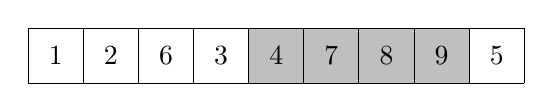
\begin{tikzpicture}[scale=0.7]
\fill[color=lightgray] (4,0) rectangle (8,1);
\draw (0,0) grid (9,1);

\node at (0.5,0.5) {$1$};
\node at (1.5,0.5) {$2$};
\node at (2.5,0.5) {$6$};
\node at (3.5,0.5) {$3$};
\node at (4.5,0.5) {$4$};
\node at (5.5,0.5) {$7$};
\node at (6.5,0.5) {$8$};
\node at (7.5,0.5) {$9$};
\node at (8.5,0.5) {$5$};
% 
% \footnotesize
% \node at (0.5,1.4) {$1$};
% \node at (1.5,1.4) {$2$};
% \node at (2.5,1.4) {$3$};
% \node at (3.5,1.4) {$4$};
% \node at (4.5,1.4) {$5$};
% \node at (5.5,1.4) {$6$};
% \node at (6.5,1.4) {$7$};
% \node at (7.5,1.4) {$8$};
% \node at (8.5,1.4) {$9$};
\end{tikzpicture}
\end{center}
با استفاده از این ویژگی، می‌توان پرسش‌های
مرتبط با زیردرخت‌های یک درخت را بهینه‌تر پردازش کرد.
به‌عنوان مثال، مسئله‌ای را در نظر بگیرید که در آن به هر گره
مقداری اختصاص داده شده است و وظیفه ما پشتیبانی
از پرسش‌های زیر است:
\begin{itemize}
\item به‌روزرسانی مقدار یک گره
\item محاسبه مجموع مقادیر در زیردرخت یک گره
\end{itemize}

درخت زیر را در نظر بگیرید که اعداد آبی‌رنگ
مقادیر گره‌ها هستند.
برای مثال، مجموع مقادیر زیردرخت گره $4$
برابر با $3+4+3+1=11$ است.

\begin{center}
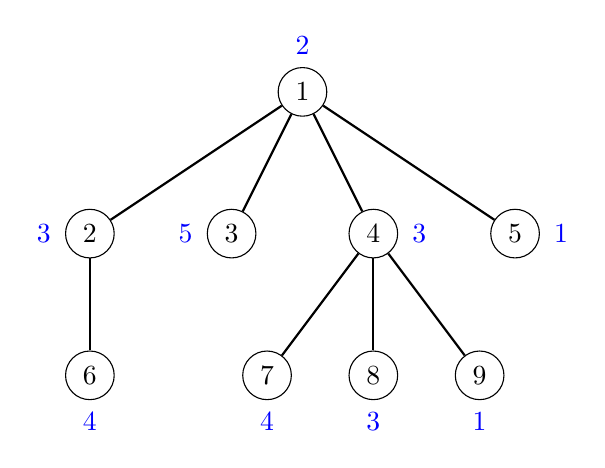
\begin{tikzpicture}[scale=0.9]
\node[draw, circle] (1) at (0,3) {$1$};
\node[draw, circle] (2) at (-3,1) {$2$};
\node[draw, circle] (3) at (-1,1) {$3$};
\node[draw, circle] (4) at (1,1) {$4$};
\node[draw, circle] (5) at (3,1) {$5$};
\node[draw, circle] (6) at (-3,-1) {$6$};
\node[draw, circle] (7) at (-0.5,-1) {$7$};
\node[draw, circle] (8) at (1,-1) {$8$};
\node[draw, circle] (9) at (2.5,-1) {$9$};

\path[draw,thick,-] (1) -- (2);
\path[draw,thick,-] (1) -- (3);
\path[draw,thick,-] (1) -- (4);
\path[draw,thick,-] (1) -- (5);
\path[draw,thick,-] (2) -- (6);
\path[draw,thick,-] (4) -- (7);
\path[draw,thick,-] (4) -- (8);
\path[draw,thick,-] (4) -- (9);

\node[color=blue] at (0,3+0.65) {2};
\node[color=blue] at (-3-0.65,1) {3};
\node[color=blue] at (-1-0.65,1) {5};
\node[color=blue] at (1+0.65,1) {3};
\node[color=blue] at (3+0.65,1) {1};
\node[color=blue] at (-3,-1-0.65) {4};
\node[color=blue] at (-0.5,-1-0.65) {4};
\node[color=blue] at (1,-1-0.65) {3};
\node[color=blue] at (2.5,-1-0.65) {1};
\end{tikzpicture}
\end{center}

ایده ساخت آرایه پیمایش درخت است شامل سه مقدار برای هر رأس: شناسه رأس، اندازه زیردرخت و مقدار رأس.
برای نمونه آرایه درخت بالا چنین است:

\begin{center}
\begin{tikzpicture}[scale=0.7]
\draw (0,1) grid (9,-2);

\node[left] at (-1,0.5) {شناسه رأس};
\node[left] at (-1,-0.5) {اندازه زیردرخت};
\node[left] at (-1,-1.5) {مقدار رأس};

\node at (0.5,0.5) {$1$};
\node at (1.5,0.5) {$2$};
\node at (2.5,0.5) {$6$};
\node at (3.5,0.5) {$3$};
\node at (4.5,0.5) {$4$};
\node at (5.5,0.5) {$7$};
\node at (6.5,0.5) {$8$};
\node at (7.5,0.5) {$9$};
\node at (8.5,0.5) {$5$};

\node at (0.5,-0.5) {$9$};
\node at (1.5,-0.5) {$2$};
\node at (2.5,-0.5) {$1$};
\node at (3.5,-0.5) {$1$};
\node at (4.5,-0.5) {$4$};
\node at (5.5,-0.5) {$1$};
\node at (6.5,-0.5) {$1$};
\node at (7.5,-0.5) {$1$};
\node at (8.5,-0.5) {$1$};

\node at (0.5,-1.5) {$2$};
\node at (1.5,-1.5) {$3$};
\node at (2.5,-1.5) {$4$};
\node at (3.5,-1.5) {$5$};
\node at (4.5,-1.5) {$3$};
\node at (5.5,-1.5) {$4$};
\node at (6.5,-1.5) {$3$};
\node at (7.5,-1.5) {$1$};
\node at (8.5,-1.5) {$1$};
% 
% \footnotesize
% \node at (0.5,1.4) {$1$};
% \node at (1.5,1.4) {$2$};
% \node at (2.5,1.4) {$3$};
% \node at (3.5,1.4) {$4$};
% \node at (4.5,1.4) {$5$};
% \node at (5.5,1.4) {$6$};
% \node at (6.5,1.4) {$7$};
% \node at (7.5,1.4) {$8$};
% \node at (8.5,1.4) {$9$};
\end{tikzpicture}
\end{center}

با استفاده از این آرایه، محاسبه مجموع مقادیر در هر زیردرخت با یافتن اندازه زیردرخت و سپس مقادیر رئوس متناظر امکان‌پذیر است.
برای نمونه مقادیر زیردرخت رأس $4$ به این صورت یافت می‌شوند:

\begin{center}
\begin{tikzpicture}[scale=0.7]
\fill[color=lightgray] (4,1) rectangle (5,0);
\fill[color=lightgray] (4,0) rectangle (5,-1);
\fill[color=lightgray] (4,-1) rectangle (8,-2);
\draw (0,1) grid (9,-2);

\node[left] at (-1,0.5) {شناسه رأس};
\node[left] at (-1,-0.5) {اندازه زیردرخت};
\node[left] at (-1,-1.5) {مقدار رأس};

\node at (0.5,0.5) {$1$};
\node at (1.5,0.5) {$2$};
\node at (2.5,0.5) {$6$};
\node at (3.5,0.5) {$3$};
\node at (4.5,0.5) {$4$};
\node at (5.5,0.5) {$7$};
\node at (6.5,0.5) {$8$};
\node at (7.5,0.5) {$9$};
\node at (8.5,0.5) {$5$};

\node at (0.5,-0.5) {$9$};
\node at (1.5,-0.5) {$2$};
\node at (2.5,-0.5) {$1$};
\node at (3.5,-0.5) {$1$};
\node at (4.5,-0.5) {$4$};
\node at (5.5,-0.5) {$1$};
\node at (6.5,-0.5) {$1$};
\node at (7.5,-0.5) {$1$};
\node at (8.5,-0.5) {$1$};

\node at (0.5,-1.5) {$2$};
\node at (1.5,-1.5) {$3$};
\node at (2.5,-1.5) {$4$};
\node at (3.5,-1.5) {$5$};
\node at (4.5,-1.5) {$3$};
\node at (5.5,-1.5) {$4$};
\node at (6.5,-1.5) {$3$};
\node at (7.5,-1.5) {$1$};
\node at (8.5,-1.5) {$1$};
% 
% \footnotesize
% \node at (0.5,1.4) {$1$};
% \node at (1.5,1.4) {$2$};
% \node at (2.5,1.4) {$3$};
% \node at (3.5,1.4) {$4$};
% \node at (4.5,1.4) {$5$};
% \node at (5.5,1.4) {$6$};
% \node at (6.5,1.4) {$7$};
% \node at (7.5,1.4) {$8$};
% \node at (8.5,1.4) {$9$};
\end{tikzpicture}
\end{center}

برای پاسخ‌دهی به پرس‌و‌جوها به صورت کارا،
ذخیره مقادیر گره‌ها در درخت ایندکس‌شده باینری یا درخت بازه‌ای کافی است.
سپس، هم به‌روزرسانی مقدار و هم محاسبه مجموع مقادیر در زمان $O(\log n)$ انجام می‌شود.

\subsubsection{پرس‌وجوهای مسیر}

با استفاده از آرایه پیمایش درخت، محاسبه کارای مجموع مقادیر روی مسیرهای از ریشه به هر گره دلخواه درخت نیز ممکن است.
مسئله‌ای را در نظر بگیرید که هدف پشتیبانی از این پرس‌وجوها است:
\begin{itemize}
\item تغییر مقدار یک گره
\item محاسبه مجموع مقادیر روی مسیر از ریشه تا یک گره
\end{itemize}

برای نمونه، در درخت زیر،
مجموع مقادیر از ریشه تا گره ۷ برابر است با
$4+5+5=14$:

\begin{center}
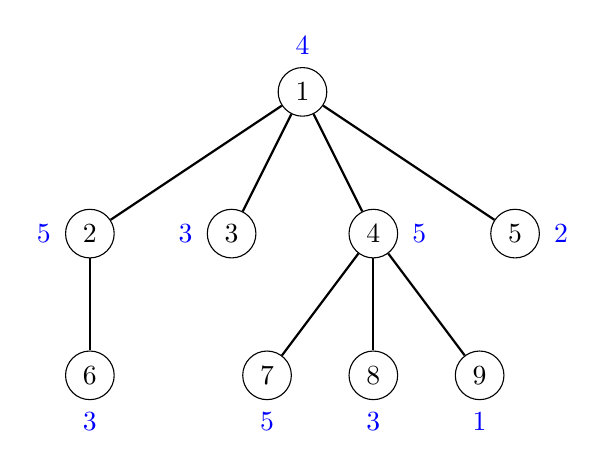
\begin{tikzpicture}[scale=0.9]
\node[draw, circle] (1) at (0,3) {$1$};
\node[draw, circle] (2) at (-3,1) {$2$};
\node[draw, circle] (3) at (-1,1) {$3$};
\node[draw, circle] (4) at (1,1) {$4$};
\node[draw, circle] (5) at (3,1) {$5$};
\node[draw, circle] (6) at (-3,-1) {$6$};
\node[draw, circle] (7) at (-0.5,-1) {$7$};
\node[draw, circle] (8) at (1,-1) {$8$};
\node[draw, circle] (9) at (2.5,-1) {$9$};

\path[draw,thick,-] (1) -- (2);
\path[draw,thick,-] (1) -- (3);
\path[draw,thick,-] (1) -- (4);
\path[draw,thick,-] (1) -- (5);
\path[draw,thick,-] (2) -- (6);
\path[draw,thick,-] (4) -- (7);
\path[draw,thick,-] (4) -- (8);
\path[draw,thick,-] (4) -- (9);

\node[color=blue] at (0,3+0.65) {4};
\node[color=blue] at (-3-0.65,1) {5};
\node[color=blue] at (-1-0.65,1) {3};
\node[color=blue] at (1+0.65,1) {5};
\node[color=blue] at (3+0.65,1) {2};
\node[color=blue] at (-3,-1-0.65) {3};
\node[color=blue] at (-0.5,-1-0.65) {5};
\node[color=blue] at (1,-1-0.65) {3};
\node[color=blue] at (2.5,-1-0.65) {1};
\end{tikzpicture}
\end{center}

حل مسئله مانند قبل ممکن است،
اما اکنون هر مقدار سطر آخر آرایه نشان‌دهنده مجموع مقادیر روی مسیر از ریشه تا گره است.
برای نمونه، آرایه زیر متناظر با درخت بالا است:
\begin{center}
\begin{tikzpicture}[scale=0.7]
\draw (0,1) grid (9,-2);

\node[left] at (-1,0.5) {شناسه گره};
\node[left] at (-1,-0.5) {اندازه زیردرخت};
\node[left] at (-1,-1.5) {مجموع مسیر};

\node at (0.5,0.5) {$1$};
\node at (1.5,0.5) {$2$};
\node at (2.5,0.5) {$6$};
\node at (3.5,0.5) {$3$};
\node at (4.5,0.5) {$4$};
\node at (5.5,0.5) {$7$};
\node at (6.5,0.5) {$8$};
\node at (7.5,0.5) {$9$};
\node at (8.5,0.5) {$5$};

\node at (0.5,-0.5) {$9$};
\node at (1.5,-0.5) {$2$};
\node at (2.5,-0.5) {$1$};
\node at (3.5,-0.5) {$1$};
\node at (4.5,-0.5) {$4$};
\node at (5.5,-0.5) {$1$};
\node at (6.5,-0.5) {$1$};
\node at (7.5,-0.5) {$1$};
\node at (8.5,-0.5) {$1$};

\node at (0.5,-1.5) {$4$};
\node at (1.5,-1.5) {$9$};
\node at (2.5,-1.5) {$12$};
\node at (3.5,-1.5) {$7$};
\node at (4.5,-1.5) {$9$};
\node at (5.5,-1.5) {$14$};
\node at (6.5,-1.5) {$12$};
\node at (7.5,-1.5) {$10$};
\node at (8.5,-1.5) {$6$};
\end{tikzpicture}
\end{center}

وقتی مقدار یک رأس به اندازه $x$ افزایش می‌یابد،
مجموع‌های تمام رئوس در زیردرخت آن نیز به اندازه $x$ افزایش می‌یابند.
به عنوان مثال، اگر مقدار رأس ۴ به اندازه ۱ افزایش یابد،
آرایه به صورت زیر تغییر می‌کند:

\begin{center}
\begin{tikzpicture}[scale=0.7]
\fill[color=lightgray] (4,-1) rectangle (8,-2);
\draw (0,1) grid (9,-2);

\node[left] at (-1,0.5) {شناسه رأس};
\node[left] at (-1,-0.5) {اندازه زیردرخت};
\node[left] at (-1,-1.5) {مجموع مسیر};

\node at (0.5,0.5) {$1$};
\node at (1.5,0.5) {$2$};
\node at (2.5,0.5) {$6$};
\node at (3.5,0.5) {$3$};
\node at (4.5,0.5) {$4$};
\node at (5.5,0.5) {$7$};
\node at (6.5,0.5) {$8$};
\node at (7.5,0.5) {$9$};
\node at (8.5,0.5) {$5$};

\node at (0.5,-0.5) {$9$};
\node at (1.5,-0.5) {$2$};
\node at (2.5,-0.5) {$1$};
\node at (3.5,-0.5) {$1$};
\node at (4.5,-0.5) {$4$};
\node at (5.5,-0.5) {$1$};
\node at (6.5,-0.5) {$1$};
\node at (7.5,-0.5) {$1$};
\node at (8.5,-0.5) {$1$};

\node at (0.5,-1.5) {$4$};
\node at (1.5,-1.5) {$9$};
\node at (2.5,-1.5) {$12$};
\node at (3.5,-1.5) {$7$};
\node at (4.5,-1.5) {$10$};
\node at (5.5,-1.5) {$15$};
\node at (6.5,-1.5) {$13$};
\node at (7.5,-1.5) {$11$};
\node at (8.5,-1.5) {$6$};
\end{tikzpicture}
\end{center}

بنابراین، برای پشتیبانی از هر دو عملیات،
باید بتوانیم مقادیر یک بازه را افزایش دهیم
و مقدار یک عضو منفرد را بازیابی کنیم.
این کار در زمان $O(\log n)$
با استفاده از درخت پدیده‌آورده دوودیی (فنویک)
یا درخت بازه‌ای امکان‌پذیر است (بخش ۹.۴ را ببینید).

\section{پایین‌ترین جد مشترک}

\index{پایین‌ترین جد مشترک}

\key{پایین‌ترین جد مشترک}
دو رأس در یک درخت ریشه‌دار، پایین‌ترین رأسی است
که زیردرخت آن شامل هر دو رأس باشد.
یک مسئله معمول، پردازش کارآمد پرسش‌هایی است
که پایین‌ترین جد مشترک دو رأس را می‌خواهند.

به عنوان مثال، در درخت زیر،
پایین‌ترین جد مشترک رئوس ۵ و ۸،
رأس ۲ است:
\begin{center}
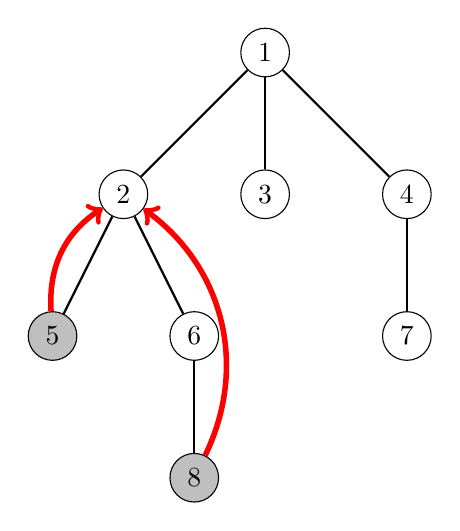
\begin{tikzpicture}[scale=0.9]
\node[draw, circle] (1) at (0,3) {$1$};
\node[draw, circle] (2) at (2,1) {$4$};
\node[draw, circle] (3) at (-2,1) {$2$};
\node[draw, circle] (4) at (0,1) {$3$};
\node[draw, circle] (5) at (2,-1) {$7$};
\node[draw, circle, fill=lightgray] (6) at (-3,-1) {$5$};
\node[draw, circle] (7) at (-1,-1) {$6$};
\node[draw, circle, fill=lightgray] (8) at (-1,-3) {$8$};
\path[draw,thick,-] (1) -- (2);
\path[draw,thick,-] (1) -- (3);
\path[draw,thick,-] (1) -- (4);
\path[draw,thick,-] (2) -- (5);
\path[draw,thick,-] (3) -- (6);
\path[draw,thick,-] (3) -- (7);
\path[draw,thick,-] (7) -- (8);

\path[draw=red,thick,->,line width=2pt] (6) edge [bend left] (3);
\path[draw=red,thick,->,line width=2pt] (8) edge [bend right=40] (3);
\end{tikzpicture}
\end{center}

در ادامه دو روش کارآمد برای یافتن کمترین جد مشترک دو رأس بررسی می‌شود.

\subsubsection{روش ۱}

یک روش حل مسئله، استفاده از امکان یافتن سریع جد $k$ام هر رأس در درخت است. با این ایده، مسئله یافتن کمترین جد مشترک به دو بخش تقسیم می‌شود.

دو اشاره‌گر به کار می‌رود که ابتدا به دو رأس هدف اشاره دارند. نخست، یکی از اشاره‌گرها به سمت بالا برده می‌شود تا هر دو اشاره‌گر روی یک سطح قرار گیرند.

در مثال فرضی، اشاره‌گر دوم یک سطح به بالا منتقل می‌شود تا به رأس ۶ برسد؛ رأسی که هم‌سطح با رأس ۵ است:

\begin{center}
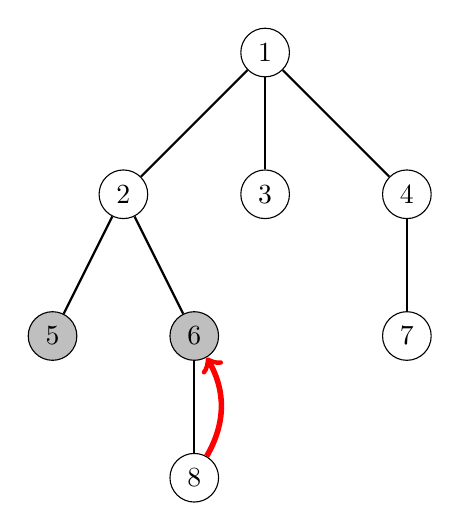
\begin{tikzpicture}[scale=0.9]
\node[draw, circle] (1) at (0,3) {$1$};
\node[draw, circle] (2) at (2,1) {$4$};
\node[draw, circle] (3) at (-2,1) {$2$};
\node[draw, circle] (4) at (0,1) {$3$};
\node[draw, circle] (5) at (2,-1) {$7$};
\node[draw, circle,fill=lightgray] (6) at (-3,-1) {$5$};
\node[draw, circle,fill=lightgray] (7) at (-1,-1) {$6$};
\node[draw, circle] (8) at (-1,-3) {$8$};
\path[draw,thick,-] (1) -- (2);
\path[draw,thick,-] (1) -- (3);
\path[draw,thick,-] (1) -- (4);
\path[draw,thick,-] (2) -- (5);
\path[draw,thick,-] (3) -- (6);
\path[draw,thick,-] (3) -- (7);
\path[draw,thick,-] (7) -- (8);

\path[draw=red,thick,->,line width=2pt] (8) edge [bend right] (7);
\end{tikzpicture}
\end{center}

سپس حداقل تعداد گام‌های لازم برای انتقال هم‌زمان هر دو اشاره‌گر به بالا، تا رسیدن به رأسی یکسان، تعیین می‌شود. رأسی که اشاره‌گرها در پایان به آن اشاره دارند، کمترین جد مشترک است.

در مثال فرضی، کافی است هر دو اشاره‌گر یک گام به بالا بروند و به رأس ۲ برسند که همان کمترین جد مشترک است:

\begin{center}
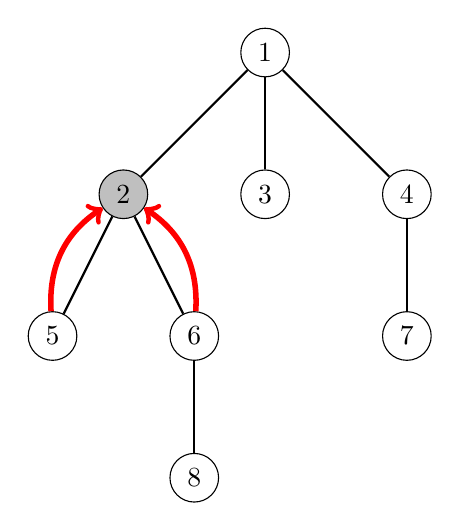
\begin{tikzpicture}[scale=0.9]
\node[draw, circle] (1) at (0,3) {$1$};
\node[draw, circle] (2) at (2,1) {$4$};
\node[draw, circle,fill=lightgray] (3) at (-2,1) {$2$};
\node[draw, circle] (4) at (0,1) {$3$};
\node[draw, circle] (5) at (2,-1) {$7$};
\node[draw, circle] (6) at (-3,-1) {$5$};
\node[draw, circle] (7) at (-1,-1) {$6$};
\node[draw, circle] (8) at (-1,-3) {$8$};
\path[draw,thick,-] (1) -- (2);
\path[draw,thick,-] (1) -- (3);
\path[draw,thick,-] (1) -- (4);
\path[draw,thick,-] (2) -- (5);
\path[draw,thick,-] (3) -- (6);
\path[draw,thick,-] (3) -- (7);
\path[draw,thick,-] (7) -- (8);

\path[draw=red,thick,->,line width=2pt] (6) edge [bend left] (3);
\path[draw=red,thick,->,line width=2pt] (7) edge [bend right] (3);
\end{tikzpicture}
\end{center}

از آنجا که هر دو بخش الگوریتم با داده‌های پیش‌محاسبه‌شده در زمان $O(\log n)$ انجام می‌شوند، کمترین جد مشترک هر دو رأس در زمان $O(\log n)$ به دست می‌آید.

\subsubsection{روش ۲}

روش دیگر برای حل مسئله بر پایه آرایه پیمایش درخت است\footnote{این الگوریتم کمترین جد مشترک در \cite{ben00} ارائه شد.
این روش گاهی \index{تکنیک تور اویلری}\key{تکنیک تور اویلری} نامیده می‌شود \cite{tar84}.}.
باز هم ایده، پیمایش گره‌ها با جستجوی اول عمق است:

\begin{center}
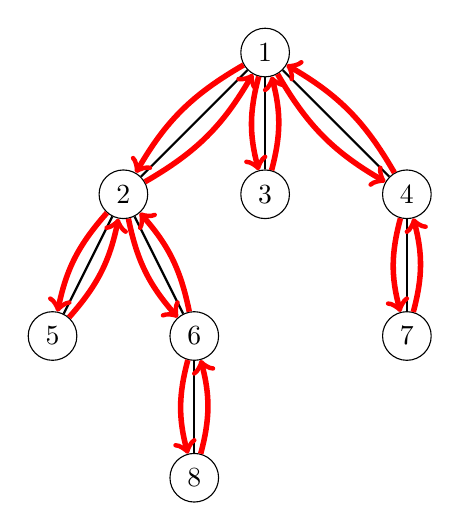
\begin{tikzpicture}[scale=0.9]
\node[draw, circle] (1) at (0,3) {$1$};
\node[draw, circle] (2) at (2,1) {$4$};
\node[draw, circle] (3) at (-2,1) {$2$};
\node[draw, circle] (4) at (0,1) {$3$};
\node[draw, circle] (5) at (2,-1) {$7$};
\node[draw, circle] (6) at (-3,-1) {$5$};
\node[draw, circle] (7) at (-1,-1) {$6$};
\node[draw, circle] (8) at (-1,-3) {$8$};
\path[draw,thick,-] (1) -- (2);
\path[draw,thick,-] (1) -- (3);
\path[draw,thick,-] (1) -- (4);
\path[draw,thick,-] (2) -- (5);
\path[draw,thick,-] (3) -- (6);
\path[draw,thick,-] (3) -- (7);
\path[draw,thick,-] (7) -- (8);

\path[draw=red,thick,->,line width=2pt] (1) edge [bend right=15] (3);
\path[draw=red,thick,->,line width=2pt] (3) edge [bend right=15] (6);
\path[draw=red,thick,->,line width=2pt] (6) edge [bend right=15] (3);
\path[draw=red,thick,->,line width=2pt] (3) edge [bend right=15] (7);
\path[draw=red,thick,->,line width=2pt] (7) edge [bend right=15] (8);
\path[draw=red,thick,->,line width=2pt] (8) edge [bend right=15] (7);
\path[draw=red,thick,->,line width=2pt] (7) edge [bend right=15] (3);
\path[draw=red,thick,->,line width=2pt] (3) edge [bend right=15] (1);
\path[draw=red,thick,->,line width=2pt] (1) edge [bend right=15] (4);
\path[draw=red,thick,->,line width=2pt] (4) edge [bend right=15] (1);
\path[draw=red,thick,->,line width=2pt] (1) edge [bend right=15] (2);
\path[draw=red,thick,->,line width=2pt] (2) edge [bend right=15] (5);
\path[draw=red,thick,->,line width=2pt] (5) edge [bend right=15] (2);
\path[draw=red,thick,->,line width=2pt] (2) edge [bend right=15] (1);
\end{tikzpicture}
\end{center}

اما از آرایه پیمایش درختی متفاوتی نسبت به قبل استفاده می‌کنیم:
هر بار که جستجوی اول عمق از گره عبور می‌کند، گره را \emph{همواره} به آرایه اضافه می‌کنیم،
نه فقط در اولین بازدید.
بنابراین گره با $k$ فرزند، $k+1$ بار در آرایه ظاهر می‌شود
و در کل $2n-1$ گره در آرایه وجود دارد.

دو مقدار در آرایه ذخیره می‌کنیم:
شناسه گره و عمق گره در درخت.
آرایه زیر متناظر با درخت بالا است:

\begin{center}
\begin{tikzpicture}[scale=0.7]

\node[left] at (-1,1.5) {شناسه گره};
\node[left] at (-1,0.5) {عمق};

\draw (0,1) grid (15,2);
\node at (0.5,1.5) {$1$};
\node at (1.5,1.5) {$2$};
\node at (2.5,1.5) {$5$};
\node at (3.5,1.5) {$2$};
\node at (4.5,1.5) {$6$};
\node at (5.5,1.5) {$8$};
\node at (6.5,1.5) {$6$};
\node at (7.5,1.5) {$2$};
\node at (8.5,1.5) {$1$};
\node at (9.5,1.5) {$3$};
\node at (10.5,1.5) {$1$};
\node at (11.5,1.5) {$4$};
\node at (12.5,1.5) {$7$};
\node at (13.5,1.5) {$4$};
\node at (14.5,1.5) {$1$};

\draw (0,0) grid (15,1);
\node at (0.5,0.5) {$1$};
\node at (1.5,0.5) {$2$};
\node at (2.5,0.5) {$3$};
\node at (3.5,0.5) {$2$};
\node at (4.5,0.5) {$3$};
\node at (5.5,0.5) {$4$};
\node at (6.5,0.5) {$3$};
\node at (7.5,0.5) {$2$};
\node at (8.5,0.5) {$1$};
\node at (9.5,0.5) {$2$};
\node at (10.5,0.5) {$1$};
\node at (11.5,0.5) {$2$};
\node at (12.5,0.5) {$3$};
\node at (13.5,0.5) {$2$};
\node at (14.5,0.5) {$1$};

\footnotesize
\node at (0.5,2.5) {$0$};
\node at (1.5,2.5) {$1$};
\node at (2.5,2.5) {$2$};
\node at (3.5,2.5) {$3$};
\node at (4.5,2.5) {$4$};
\node at (5.5,2.5) {$5$};
\node at (6.5,2.5) {$6$};
\node at (7.5,2.5) {$7$};
\node at (8.5,2.5) {$8$};
\node at (9.5,2.5) {$9$};
\node at (10.5,2.5) {$10$};
\node at (11.5,2.5) {$11$};
\node at (12.5,2.5) {$12$};
\node at (13.5,2.5) {$13$};
\node at (14.5,2.5) {$14$};
\end{tikzpicture}
\end{center}

اکنون می‌توان کمترین نیاکان مشترک
گره‌های $a$ و $b$ را با یافتن گره دارای \emph{کمینه} عمق
بین گره‌های $a$ و $b$ در آرایه پیدا کرد.
برای نمونه، کمترین نیاکان مشترک گره‌های $5$ و $8$
به صورت زیر یافت می‌شود:

\begin{center}
\begin{tikzpicture}[scale=0.7]

\node[left] at (-1,1.5) {شناسه گره};
\node[left] at (-1,0.5) {عمق};

\fill[color=lightgray] (2,1) rectangle (3,2);
\fill[color=lightgray] (5,1) rectangle (6,2);
\fill[color=lightgray] (2,0) rectangle (6,1);

\node at (3.5,-0.5) {$\uparrow$};

\draw (0,1) grid (15,2);
\node at (0.5,1.5) {$1$};
\node at (1.5,1.5) {$2$};
\node at (2.5,1.5) {$5$};
\node at (3.5,1.5) {$2$};
\node at (4.5,1.5) {$6$};
\node at (5.5,1.5) {$8$};
\node at (6.5,1.5) {$6$};
\node at (7.5,1.5) {$2$};
\node at (8.5,1.5) {$1$};
\node at (9.5,1.5) {$3$};
\node at (10.5,1.5) {$1$};
\node at (11.5,1.5) {$4$};
\node at (12.5,1.5) {$7$};
\node at (13.5,1.5) {$4$};
\node at (14.5,1.5) {$1$};


\draw (0,0) grid (15,1);
\node at (0.5,0.5) {$1$};
\node at (1.5,0.5) {$2$};
\node at (2.5,0.5) {$3$};
\node at (3.5,0.5) {$2$};
\node at (4.5,0.5) {$3$};
\node at (5.5,0.5) {$4$};
\node at (6.5,0.5) {$3$};
\node at (7.5,0.5) {$2$};
\node at (8.5,0.5) {$1$};
\node at (9.5,0.5) {$2$};
\node at (10.5,0.5) {$1$};
\node at (11.5,0.5) {$2$};
\node at (12.5,0.5) {$3$};
\node at (13.5,0.5) {$2$};
\node at (14.5,0.5) {$1$};

\footnotesize
\node at (0.5,2.5) {$0$};
\node at (1.5,2.5) {$1$};
\node at (2.5,2.5) {$2$};
\node at (3.5,2.5) {$3$};
\node at (4.5,2.5) {$4$};
\node at (5.5,2.5) {$5$};
\node at (6.5,2.5) {$6$};
\node at (7.5,2.5) {$7$};
\node at (8.5,2.5) {$8$};
\node at (9.5,2.5) {$9$};
\node at (10.5,2.5) {$10$};
\node at (11.5,2.5) {$11$};
\node at (12.5,2.5) {$12$};
\node at (13.5,2.5) {$13$};
\node at (14.5,2.5) {$14$};
\end{tikzpicture}
\end{center}

گره ۵ در موقعیت ۲، گره ۸ در موقعیت ۵ قرار دارد
و گره با کمینه عمق بین
موقعیت‌های $2 \ldots 5$ گره ۲ در موقعیت ۳ است
که عمق آن ۲ می‌باشد.
بنابراین، کمترین نیاکان مشترک
گره‌های ۵ و ۸، گره ۲ است.

بنابراین، برای یافتن کمترین نیاکان مشترک
دو رأس، پردازش یک پرس‌وجوی کمینه بازه کافی است.
از آنجا که آرایه ایستا است،
می‌توان این پرس‌وجوها را در زمان $O(1)$
پس از پیش‌پردازشی با زمان $O(n \log n)$ پاسخ داد.

\subsubsection{فاصله رأس‌ها}

فاصله بین دو رأس $a$ و $b$
برابر طول مسیر از $a$ به $b$ است.
مشخص می‌شود که مسئله محاسبه
فاصله بین رأس‌ها به یافتن
کمترین نیاکان مشترک آن‌ها کاهش می‌یابد.

ابتدا، درخت را به دلخواه ریشه‌دار می‌کنیم.
سپس، فاصله رأس‌های $a$ و $b$
با استفاده از این فرمول محاسبه می‌شود:
\[\texttt{depth}(a)+\texttt{depth}(b)-2 \cdot \texttt{depth}(c),\]
که در آن $c$ کمترین نیاکان مشترک $a$ و $b$ است
و $\texttt{depth}(s)$ عمق رأس $s$ را نشان می‌دهد.
برای مثال، فاصله رأس‌های 5 و 8 را در نظر بگیرید:
\begin{center}
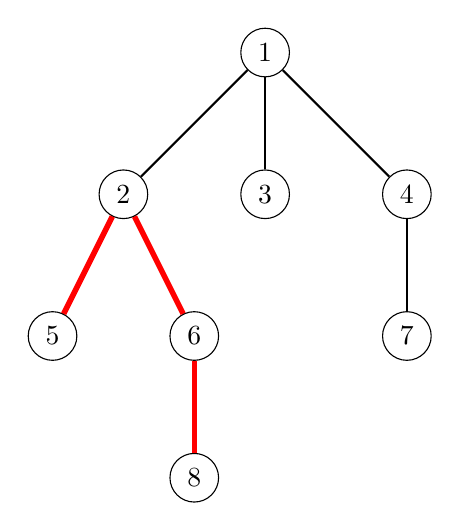
\begin{tikzpicture}[scale=0.9]
\node[draw, circle] (1) at (0,3) {$1$};
\node[draw, circle] (2) at (2,1) {$4$};
\node[draw, circle] (3) at (-2,1) {$2$};
\node[draw, circle] (4) at (0,1) {$3$};
\node[draw, circle] (5) at (2,-1) {$7$};
\node[draw, circle] (6) at (-3,-1) {$5$};
\node[draw, circle] (7) at (-1,-1) {$6$};
\node[draw, circle] (8) at (-1,-3) {$8$};
\path[draw,thick,-] (1) -- (2);
\path[draw,thick,-] (1) -- (3);
\path[draw,thick,-] (1) -- (4);
\path[draw,thick,-] (2) -- (5);
\path[draw,thick,-] (3) -- (6);
\path[draw,thick,-] (3) -- (7);
\path[draw,thick,-] (7) -- (8);

\path[draw=red,thick,-,line width=2pt] (8) -- node[font=\small] {} (7);
\path[draw=red,thick,-,line width=2pt] (7) -- node[font=\small] {} (3);
\path[draw=red,thick,-,line width=2pt] (6) -- node[font=\small] {} (3);
\end{tikzpicture}
\end{center}

کمترین نیاکان مشترک رأس‌های 5 و 8 رأس 2 است.
عمق این رأس‌ها عبارت است از:
$\texttt{depth}(5)=3$، $\texttt{depth}(8)=4$ و $\texttt{depth}(2)=2$،
بنابراین فاصله بین رأس‌های 5 و 8 برابر است با:
$3+4-2\cdot2=3$.

\section{الگوریتم‌های برون‌خط}

تا اینجا، الگوریتم‌های \emph{برخط}
برای پرس‌وجوهای درخت را بررسی کردیم.
این الگوریتم‌ها پرس‌وجوها را پی‌درپی پردازش می‌کنند،
به طوری که پاسخ هر پرس‌وجو پیش از دریافت پرس‌وجوی بعدی داده می‌شود.

با این حال، در بسیاری از مسائل، ویژگی
برخط بودن الزامی نیست.
در این بخش، بر الگوریتم‌های \emph{برون‌خط} تمرکز می‌کنیم.
به این الگوریتم‌ها مجموعه‌ای از پرس‌وجوها داده می‌شود که می‌توان
آن‌ها را به هر ترتیبی پاسخ داد.
طراحی یک الگوریتم برون‌خط معمولاً آسان‌تر
از یک الگوریتم برخط است.

\subsubsection{ادغام ساختمان داده‌ها}

یک روش برای ساخت الگوریتم برون‌خط،
پیمایش اول‌سطح یا اول‌عمق درخت
و نگهداری ساختمان داده‌ها در رأس‌ها است.
در هر رأس $s$، ساختمان داده
$\texttt{d}[s]$ بر پایه ساختمان داده‌های
فرزندان $s$ ایجاد می‌شود.
سپس با استفاده از این ساختمان داده،
تمام پرس‌وجوهای مربوط به $s$ پردازش می‌شوند.

به عنوان مثال، مسئله زیر را در نظر بگیرید:
درختی داده شده است که هر راس مقداری دارد.
هدف، پاسخ به پرسش‌هایی به این صورت است:
«تعداد راس‌های با مقدار $x$
در زیردرخت راس $s$ را محاسبه کنید».
برای نمونه، در درخت زیر،
زیردرخت راس $4$ شامل دو راس
با مقدار 3 است.

\begin{center}
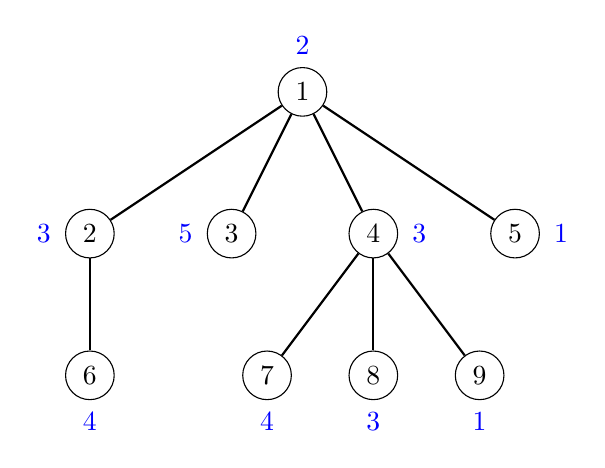
\begin{tikzpicture}[scale=0.9]
\node[draw, circle] (1) at (0,3) {$1$};
\node[draw, circle] (2) at (-3,1) {$2$};
\node[draw, circle] (3) at (-1,1) {$3$};
\node[draw, circle] (4) at (1,1) {$4$};
\node[draw, circle] (5) at (3,1) {$5$};
\node[draw, circle] (6) at (-3,-1) {$6$};
\node[draw, circle] (7) at (-0.5,-1) {$7$};
\node[draw, circle] (8) at (1,-1) {$8$};
\node[draw, circle] (9) at (2.5,-1) {$9$};

\path[draw,thick,-] (1) -- (2);
\path[draw,thick,-] (1) -- (3);
\path[draw,thick,-] (1) -- (4);
\path[draw,thick,-] (1) -- (5);
\path[draw,thick,-] (2) -- (6);
\path[draw,thick,-] (4) -- (7);
\path[draw,thick,-] (4) -- (8);
\path[draw,thick,-] (4) -- (9);

\node[color=blue] at (0,3+0.65) {2};
\node[color=blue] at (-3-0.65,1) {3};
\node[color=blue] at (-1-0.65,1) {5};
\node[color=blue] at (1+0.65,1) {3};
\node[color=blue] at (3+0.65,1) {1};
\node[color=blue] at (-3,-1-0.65) {4};
\node[color=blue] at (-0.5,-1-0.65) {4};
\node[color=blue] at (1,-1-0.65) {3};
\node[color=blue] at (2.5,-1-0.65) {1};
\end{tikzpicture}
\end{center}

در این مسئله، می‌توان از ساختارهای نگاشت (map)
برای پاسخ به پرسش‌ها استفاده کرد.
به عنوان مثال، نگاشت‌های مربوط به راس 4 و
فرزندان آن بدین صورت است:

\begin{center}
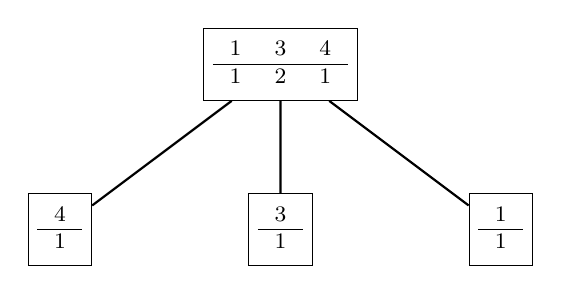
\begin{tikzpicture}[scale=0.7]

\node[draw, rectangle] (a) at (4,5.5)
{
\footnotesize
\begin{tabular}{rrr}
4 \\
\hline
1 \\
\end{tabular}};

\node[draw, rectangle] (b) at (8,5.5)
{
\footnotesize
\begin{tabular}{rrr}
3 \\
\hline
1 \\
\end{tabular}};


\node[draw, rectangle] (c) at (12,5.5)
{
\footnotesize
\begin{tabular}{rr}
1 \\
\hline
1 \\
\end{tabular}};

\node[draw, rectangle] (d) at (8,8.5)
{
\footnotesize
\begin{tabular}{rrr}
1 & 3 & 4 \\
\hline
1 & 2 & 1 \\
\end{tabular}};
\path[draw,thick,-] (a) -- (d);
\path[draw,thick,-] (b) -- (d);
\path[draw,thick,-] (c) -- (d);
\end{tikzpicture}
\end{center}

اگر چنین داده‌ساختاری برای هر راس بسازیم،
پردازش تمام پرسش‌های داده‌شده آسان است،
زیرا می‌توان همه پرسش‌های مربوط
به یک راس را بلافاصله پس از ساخت
داده‌ساختار آن پاسخ داد. برای مثال، ساختار
نگاشت بالا برای راس 4
نشان می‌دهد زیردرخت آن
شامل دو راس با مقدار 3 است.

اما ساخت تمام داده‌ساختارها از ابتدا بسیار کند خواهد بود.
در عوض، در هر راس $s$،
یک داده‌ساختار اولیه $\texttt{d}[s]$ می‌سازیم
که فقط شامل مقدار $s$ است.
سپس فرزندان $s$ را پیمایش کرده و
$\texttt{d}[s]$ را با تمام داده‌ساختارهای
$\texttt{d}[u]$ که $u$ فرزند $s$ است، \emph{ادغام} می‌کنیم.

برای مثال، در درخت بالا، نگاشت
راس $4$ با ادغام نگاشت‌های زیر ساخته می‌شود:

\begin{center}
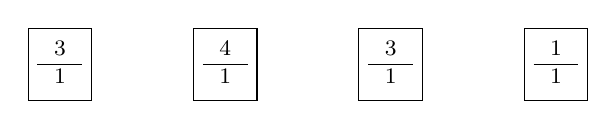
\begin{tikzpicture}[scale=0.7]

\node[draw, rectangle] (a) at (4,5.5)
{
\footnotesize
\begin{tabular}{rrr}
4 \\
\hline
1 \\
\end{tabular}};

\node[draw, rectangle] (b) at (7,5.5)
{
\footnotesize
\begin{tabular}{rrr}
3 \\
\hline
1 \\
\end{tabular}};

\node[draw, rectangle] (c) at (10,5.5)
{
\footnotesize
\begin{tabular}{rr}
1 \\
\hline
1 \\
\end{tabular}};

\node[draw, rectangle] (d) at (1,5.5)
{
\footnotesize
\begin{tabular}{rr}
3 \\
\hline
1 \\
\end{tabular}};

\end{tikzpicture}
\end{center}

در اینجا، مَپ اول ساختمان داده اولیه
برای رأس ۴ است،
و سه مَپ دیگر مربوط به رئوس ۷، ۸ و ۹ هستند.

ادغام در رأس $s$ می‌تواند به شکل زیر انجام شود:
فرزندان $s$ را پیمایش می‌کنیم
و در هر فرزند $u$، مقادیر $\texttt{d}[s]$
و $\texttt{d}[u]$ را ادغام می‌کنیم.
همیشه محتویات را از $\texttt{d}[u]$
به $\texttt{d}[s]$ کپی می‌کنیم.
با این حال، پیش از این کار، در صورتی که $\texttt{d}[s]$ کوچک‌تر از $\texttt{d}[u]$ باشد،
محتویات $\texttt{d}[s]$ و $\texttt{d}[u]$ را \emph{جابه‌جا (swap)} می‌کنیم.
با این روش، هر مقدار در طول پیمایش درخت تنها $O(\log n)$
بار کپی می‌شود
که کارایی الگوریتم را تضمین می‌کند.

برای جابه‌جایی بهینه محتویات دو ساختمان داده $a$ و $b$،
کافی است از کد زیر استفاده کنیم:
\begin{lstlisting}
swap(a,b);
\end{lstlisting}
تضمین می‌شود که کد بالا در صورتی که $a$ و $b$ از ساختمان داده‌های کتابخانه استاندارد C++ باشند، در زمان ثابت اجرا می‌شود.

\subsubsection{کمترین نیاکان مشترک}

یک الگوریتم برون‌خط (offline) نیز
برای پردازش مجموعه‌ای از
پرسش‌های کمترین نیاکان مشترک وجود دارد\footnote{این
الگوریتم توسط آر. ای. تارجان (R. E. Tarjan) در سال ۱۹۷۹ منتشر شد \cite{tar79}.}.
این الگوریتم بر پایه ساختمان داده مجموعه‌های مجزا (union-find) کار می‌کند
(بخش ۱۵.۲ را ببینید)، و مزیت آن
پیاده‌سازی ساده‌تر نسبت به
الگوریتم‌های بررسی‌شده قبلی در این فصل است.

الگوریتم مجموعه‌ای از جفت‌های رئوس را به عنوان ورودی دریافت می‌کند
و برای هر جفت، کمترین نیاکان مشترک آن‌ها را مشخص می‌سازد.
الگوریتم یک پیمایش اول‌عمق روی درخت انجام می‌دهد
و مجموعه‌های مجزایی از رئوس را نگهداری می‌کند.
در ابتدا، هر رأس متعلق به یک مجموعه مجزاست.
برای هر مجموعه، بالاترین رأس درخت
که به آن مجموعه تعلق دارد را نیز ذخیره می‌کنیم.

هنگامی که الگوریتم یک رأس $x$ را ملاقات می‌کند،
تمامی رئوس $y$ را بررسی می‌کند که
کمترین نیاکان مشترک $x$ و $y$
باید برای آن‌ها پیدا شود.
اگر $y$ قبلاً ملاقات شده باشد،
الگوریتم گزارش می‌دهد که 
کمترین نیاکان مشترک $x$ و $y$
همان بالاترین رأس در مجموعه $y$ است.
سپس، پس از پردازش رأس $x$،
الگوریتم مجموعه‌های $x$ و والد آن را ادغام می‌کند.

برای مثال، فرض کنید می‌خواهیم کمترین جد مشترک جفت‌راس‌های $(5,8)$ و $(2,7)$ را در درخت زیر پیدا کنیم:
\begin{center}
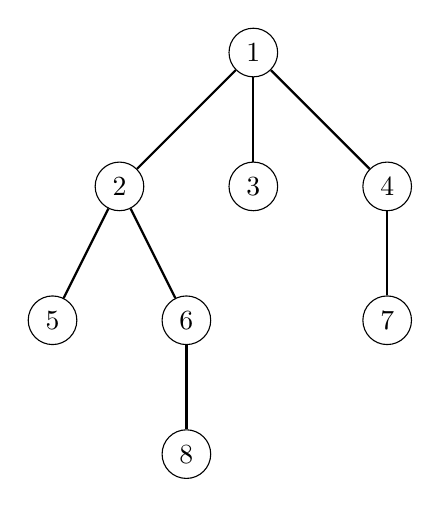
\begin{tikzpicture}[scale=0.85]
\node[draw, circle] (1) at (0,3) {$1$};
\node[draw, circle] (2) at (2,1) {$4$};
\node[draw, circle] (3) at (-2,1) {$2$};
\node[draw, circle] (4) at (0,1) {$3$};
\node[draw, circle] (5) at (2,-1) {$7$};
\node[draw, circle] (6) at (-3,-1) {$5$};
\node[draw, circle] (7) at (-1,-1) {$6$};
\node[draw, circle] (8) at (-1,-3) {$8$};
\path[draw,thick,-] (1) -- (2);
\path[draw,thick,-] (1) -- (3);
\path[draw,thick,-] (1) -- (4);
\path[draw,thick,-] (2) -- (5);
\path[draw,thick,-] (3) -- (6);
\path[draw,thick,-] (3) -- (7);
\path[draw,thick,-] (7) -- (8);
\end{tikzpicture}
\end{center}

در درخت‌های زیر، رأس‌های خاکستری نشان‌دهنده رأس‌های پیمایش‌شده هستند و دسته‌های خط‌چین رأس‌های متعلق به یک مجموعه را مشخص می‌کنند. وقتی الگوریتم به رأس 8 می‌رسد، متوجه می‌شود رأس 5 قبلاً پیمایش شده و بالاترین رأس در مجموعه آن، رأس 2 است. بنابراین، کمترین جد مشترک رأس‌های 5 و 8 برابر 2 است:
\begin{center}
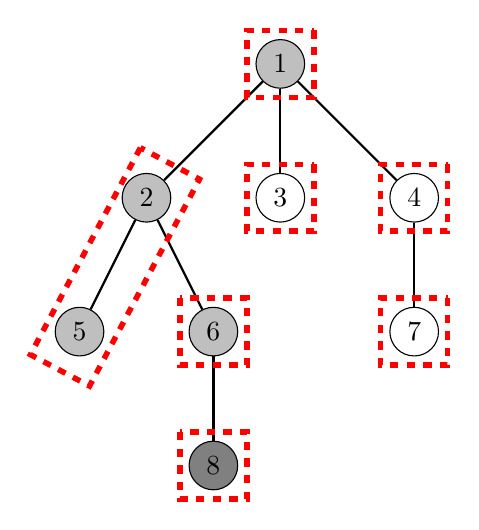
\begin{tikzpicture}[scale=0.85]
\node[draw, circle, fill=lightgray] (1) at (0,3) {$1$};
\node[draw, circle] (2) at (2,1) {$4$};
\node[draw, circle, fill=lightgray] (3) at (-2,1) {$2$};
\node[draw, circle] (4) at (0,1) {$3$};
\node[draw, circle] (5) at (2,-1) {$7$};
\node[draw, circle, fill=lightgray] (6) at (-3,-1) {$5$};
\node[draw, circle, fill=lightgray] (7) at (-1,-1) {$6$};
\node[draw, circle, fill=gray] (8) at (-1,-3) {$8$};
\path[draw,thick,-] (1) -- (2);
\path[draw,thick,-] (1) -- (3);
\path[draw,thick,-] (1) -- (4);
\path[draw,thick,-] (2) -- (5);
\path[draw,thick,-] (3) -- (6);
\path[draw,thick,-] (3) -- (7);
\path[draw,thick,-] (7) -- (8);

\draw [red,thick,dashed,line width=2pt,rotate around={-28:(-2,0)}] (-2.9,1.5) rectangle (-1.9,-2);


\draw [red,thick,dashed,line width=2pt] (-1.5,-0.5) rectangle (-0.5,-1.5);
\draw [red,thick,dashed,line width=2pt] (-1.5,-2.5) rectangle (-0.5,-3.5);

\draw [red,thick,dashed,line width=2pt] (0.5,3.5) rectangle (-0.5,2.5);
\draw [red,thick,dashed,line width=2pt] (0.5,1.5) rectangle (-0.5,0.5);
\draw [red,thick,dashed,line width=2pt] (2.5,1.5) rectangle (1.5,0.5);
\draw [red,thick,dashed,line width=2pt] (2.5,-0.5) rectangle (1.5,-1.5);
\end{tikzpicture}
\end{center}

سپس، هنگام پیمایش گره 7،
الگوریتم تعیین می‌کند که
کمترین جد مشترک گره‌های 2 و 7 برابر 1 است:
\begin{center}
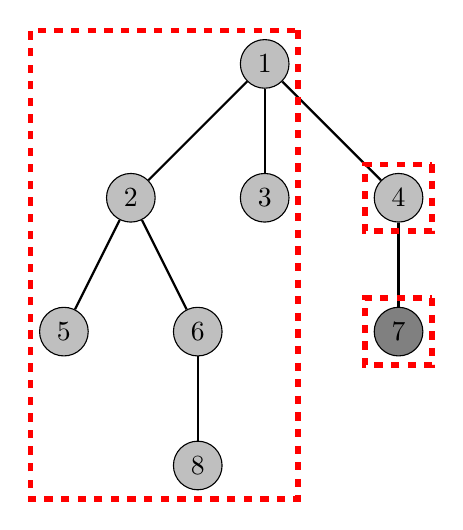
\begin{tikzpicture}[scale=0.85]
\node[draw, circle, fill=lightgray] (1) at (0,3) {$1$};
\node[draw, circle, fill=lightgray] (2) at (2,1) {$4$};
\node[draw, circle, fill=lightgray] (3) at (-2,1) {$2$};
\node[draw, circle, fill=lightgray] (4) at (0,1) {$3$};
\node[draw, circle, fill=gray] (5) at (2,-1) {$7$};
\node[draw, circle, fill=lightgray] (6) at (-3,-1) {$5$};
\node[draw, circle, fill=lightgray] (7) at (-1,-1) {$6$};
\node[draw, circle, fill=lightgray] (8) at (-1,-3) {$8$};
\path[draw,thick,-] (1) -- (2);
\path[draw,thick,-] (1) -- (3);
\path[draw,thick,-] (1) -- (4);
\path[draw,thick,-] (2) -- (5);
\path[draw,thick,-] (3) -- (6);
\path[draw,thick,-] (3) -- (7);
\path[draw,thick,-] (7) -- (8);

\draw [red,thick,dashed,line width=2pt] (0.5,3.5) rectangle (-3.5,-3.5);
\draw [red,thick,dashed,line width=2pt] (2.5,1.5) rectangle (1.5,0.5);
\draw [red,thick,dashed,line width=2pt] (2.5,-0.5) rectangle (1.5,-1.5);

\end{tikzpicture}
\end{center}